
\chapter{Gestione database}

\section{Salvataggio configurazione}

Premendo "Salva configurazione nel Database" viene aperta una finestra di dialogo dove inserire il
nome della nuova configurazione personalizzata:

\begin{figure}[H]
\centering
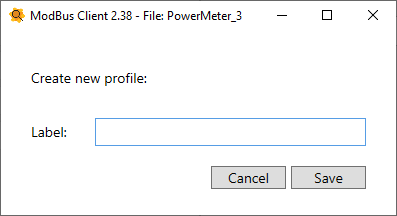
\includegraphics[width=0.3\textwidth]{../Img/SaveProfile.PNG}
\caption{Salva nuovo profilo}
\end{figure}

Premendo "Salva" all'interno della cartella "Json" viene creata una cartella con il nome inserito
nella finestra. NON sovrascrivere cartelle esistenti, per apportare modifiche ad una configurazione
personalizzata è sufficiente aprirla, le modifiche verranno salvate automaticamente alla chiusura
della finestra principale (eventualmente l'utente può salvare lo stato attuale dal menu File->Salva)

\section{Percorso configurazione}

Nella cartella "Json" sono presenti le cartelle contenenti le configurazioni personalizzate, una cartella
per ogni profilo inserito. La
cartella "Default" contiene la configurazione del programma quando non vengono utilizzate
configurazioni personalizzate (se si utilizza il programma senza caricare un profilo, ogni
modifica viene salvata in questa cartella). Le altre cartelle vengono generate quando si salva la
configurazione attuale come un nuovo profilo.

\begin{figure}[H]
\centering
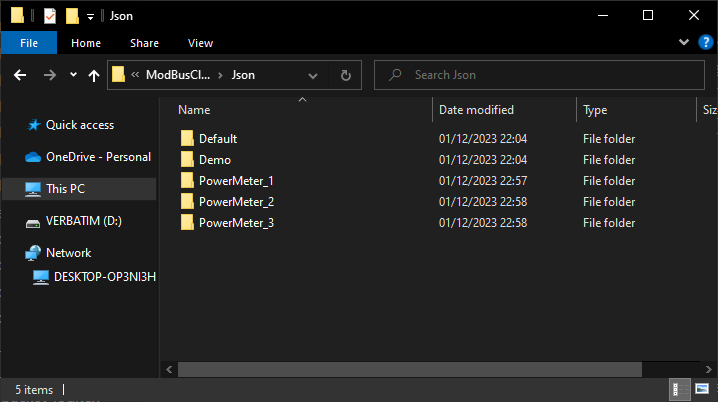
\includegraphics[width=0.45\textwidth]{../Img/DatabaseDirectory.PNG}
\caption{Directory profili database}
\end{figure}

L'utente nell'uso normale non ha bisogno di apportare modifiche direttamente in questa cartella, 
è sufficiente usare i form per salvare e caricare i profili direttamente dalla finestra principale.

\newpage
\section{Caricamento configurazione}

Premendo "Carica configurazione dal Database" è possibile caricare una configurazione
personalizzata precedentemente salvata:

\begin{figure}[H]
\centering
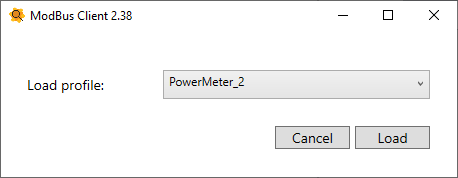
\includegraphics[width=0.45\textwidth]{../Img/LoadProfile.PNG}
\caption{Carica profilo}
\end{figure}

Una volta caricata una configurazione personalizzata qualsiasi modifica inserita nel programma
verrà salvata nella cartella personalizzata senza modificare la struttura della configurazione
"Default".

Per importare o esportare un Profilo personalizzato utilizzare il tool "Manage database",
qui è possibile esportare un profilo come file .zip, importare un profilo 
esportato da un altro client o semplicemente selezionare il profilo da caricare.
Quando si chiude la finestra viene caricato nel client 
il profilo attualmente selezionato.

\begin{figure}[H]
\centering
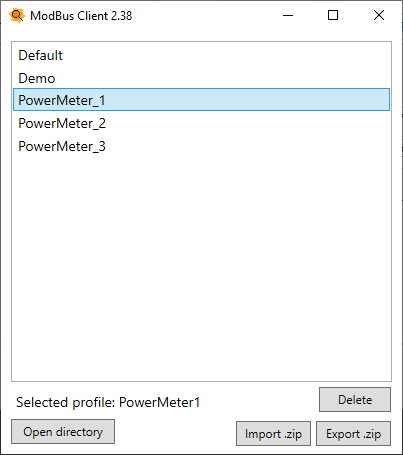
\includegraphics[width=0.40\textwidth]{../Img/DatabaseManager.PNG}
\caption{Database manager}
\end{figure}

A partire dalla versione v2.37 i profili possono essere caricati 
direttamente nella tab home tramite l'apposito menu a tendina:

\begin{figure}[H]
\centering
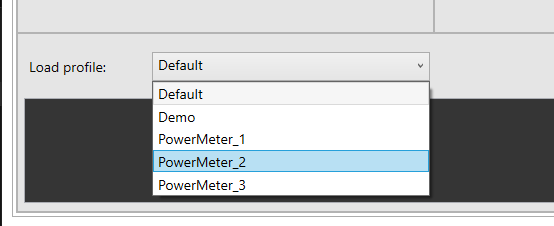
\includegraphics[width=0.50\textwidth]{../Img/ProfileHome.PNG}
\caption{Selezione profilo homepage}
\end{figure}